\documentclass{standalone}
%\pagenumbering{gobble}


%%%%%%%%%%%%%%%%%%%%%%%%%%%%%%%%%%%%%%%%%%%%
%
% schematic of magnetic field lines
% showing tension and pressure forces
%
%%%%%%%%%%%%%%%%%%%%%%%%%%%%%%%%%%%%%%%%%%%%


\usepackage{tikz}
\usetikzlibrary{arrows.meta}


\begin{document}

\newcommand\wave[1]{
	\draw[thick, xshift=#1] (0,-4) to [out=30,in=-60] (0,-2.5)
	to [out=120,in=-150] (0,-0.5) to [out=30,in=-60] (0,2)
	to [out=120,in=-150] (0,4.5);
	}

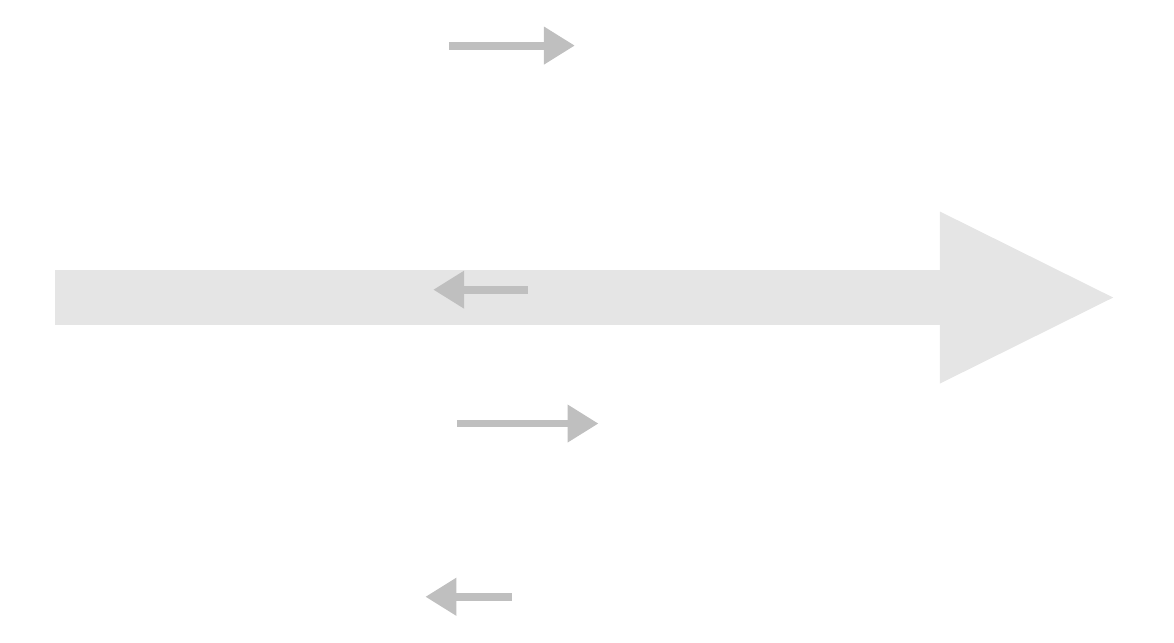
\begin{tikzpicture}[scale=1.0, font=\sffamily]

	% draw the pressure forces
	%\draw[thick, line width=1cm, color=gray!20, -triangle 60] (0,0.3) -- (13,0.3);
	\draw[line width=0.7cm, color=gray!20, arrows={-Triangle[width=2.0cm]}] (-0.5,0.3) -- (13,0.3);

	% draw the tension forces
	\draw[line width=1mm, color=gray!50, arrows={-Triangle}] (4.5,3.5) -- (6.1,3.5);
	\draw[line width=1mm, color=gray!50, arrows={-Triangle}] (5.5,0.4) -- (4.3,0.4);
	\draw[line width=1mm, color=gray!50, arrows={-Triangle}] (4.6,-1.3) -- (6.4,-1.3);
	\draw[line width=1mm, color=gray!50, arrows={-Triangle}] (5.3,-3.5) -- (4.2,-3.5);

	% draw the field lines
	\wave{0}
	\wave{0.75cm}
	\wave{2cm}
	\wave{5cm}
	\wave{9cm}

\end{tikzpicture}

\end{document} 
